\chapter{Background and Previous Work}\label{previous_work}
#TODO write a summary of the newest techniques and inventions in the field of twitter research related to finance. 
#TODO read and rewrite this chapter. 

Somewhat a starting point for this thesis:
\url{http://www.cs.ucr.edu/~vagelis/publications/wsdm2012-microblog-financial.pdf}

#TODO writer outline of this chapter. 

\section{Twitter}
Twitter is a social and information network. 
It's a real-time service for sharing and gathering small messages. These
messages can represent everything form a persons opinion of ice cream, to the
latest changes in the financial market or pictures from a Mars rover. 

At the core of Twitter you have the Tweet. The Tweet is the 140 character
message. These small pieces of information combined are the life line of Twitter.
Tweets lets you communicate with other users, share photos and post all kinds of
information. The small size of the tweets are not a hindrance for the flow of
information. 
\footnote{About Twitter: \url{https://twitter.com/about}}

The fast growing messaging service handles 1.6 billion search queries every day.
As of 2012 the 500 million users would generate 3.2 queries each on any given
day. 340 million tweets were posted every day. 
\footnote{Wikipedia: \url{http://en.wikipedia.org/wiki/Twitter}} 

Most medium and large companies have a presence on Twitter today. Posts can contain
any type of information, from promotional content to service status to
financial reports. \cite[p8]{annikajubbega11:twitter_driver_stock_price} says
that 77 of the Fortune 100 companies have a twitter account. 

Companies use twitter for feedback and customer relations. Questions can be
asked with a specific hashtag. Or with an at sign to target a specific user. This makes it easy to filter
the messages, and therefore easier to get in contact with the customer. Best
Buy demonstrated the successfulness of twitter in customer relations by
answering questions with a specific hashtag. In 2009 they had answered nearly
20 thousand questions using twitter. \cite[p1]{Li2013206}
Market Intelligence is also a major aspect of the microbloggin sphere.

Twitter represents one of the largest and most dynamic datasets of user
generated content. Along with Facebook twitter data is in real time. This has major
implications for anyone who are interested in sentiment, public opinion or
customer interaction. \cite[]{sperious11}

A typical tweet contains about 11 words and provides an opinion or state of
mind or a piece of information. Tweets can contain hashtags: #something, user:
@username, or other adaptations of prefixes such as \$STO which represents a
stock. The different prefixes or tags (\$, \#, @) easily distinguishes the
content of the tweet. This also makes it easier to search and classify the
content of tweets. Examples of tweets can be found in figure:\ref{fig:sto} and
figure:\ref{fig:tweet1}.

The retrieval of tweets seems like a challenge and impractical with
a web scraper. But Twitter has made this easy by providing an API
\footnote{API: Application programming interface}. With the API you can write
tweets and update the status of a user. But the best part of the API is that it
provides search capabilities. To get a certain subset of all tweets, we can use
the search function and view only the tweets we want. 

On the front page of twitter we have the search function at the top right of
the page. The search provides the ability to specify which types of tweets you
want. And gives you the opportunity to find the information you are looking for. 

\begin{figure}[htb]
    \centering
    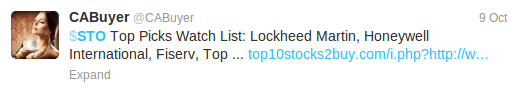
\includegraphics[width=\textwidth]{STO} 
    \caption{Typical tweet from Twitter.}
    \label{fig:sto}
\end{figure}

%\begin{figure}[htb]
%    \centering
%    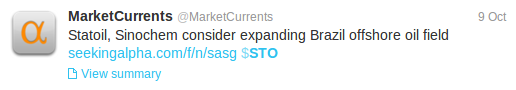
\includegraphics[width=\textwidth]{STO2} 
%    \caption{The text that shows under the image, image text.}
%    \label{fig:sto2}
%\end{figure}

\begin{figure}[htb]
    \centering
    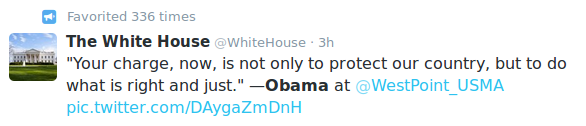
\includegraphics[width=\textwidth]{tweet1} 
    \caption{Typical tweet from Twitter.}
    \label{fig:tweet1}
\end{figure}

%\begin{figure}[htb]
%    \centering
%    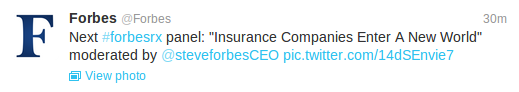
\includegraphics[width=\textwidth]{tweet2} 
%    \caption{The text that shows under the image, image text.}
%    \label{fig:tweet2}
%\end{figure}
%
%\begin{figure}[htb]
%    \centering
%    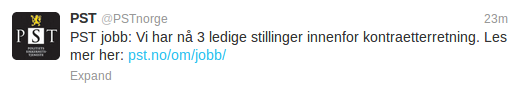
\includegraphics[width=\textwidth]{tweet3} 
%    \caption{The text that shows under the image, image text.}
%    \label{fig:tweet3}
%\end{figure}

\section{Sentiment}

Opinion mining on the web is not a new phenomenon. But in resent years it has
become much more attractive to traders in the financial world. The usage of
Twitter and other social media platforms is increasing. This means a surplus of raw data with
easy access. Companies all over the world has started to use the social
networks to their benefit. The use of information from social media has become
part of the trend, although there are some drawbacks and shortcomings. Noise and
garbage is one of them. The difficulty of the huge amount of available data is
that it's difficult to find only the information relevant for your use. Even if you're right 80\% of
the time, the last 20\% can prove devastating.
\cite[]{stevenson12:social_media_stock_pickers}

Sentiment broadly refers to a persons state of mind. Based on the state of mind the person will do optimistic or
pessimistic choices. A positive state of mind leads to optimistic judgements of
future events, and a negative state of mind leads to pessimistic.
\cite[p4]{doukas10:sentiment_and_momentum}

The users may have different roles and intentions in different
communities in the microblogging sphere, \cite[]{java07}. 
A users intentions and its reasons for participation might be a factor in the sentiment analysis.

\subsection{What is Sentiment Analysis}
There are two main categories of approaches to sentiment analysis. 
	The first is to use a classifier. The classifier can use methods such as
naive Byes, maximum entropy or support vector model \cite[]{Li2013206} This is
typically a method where it would be natural to use machine learning of
evolutionary algorithms to increase the classification correctness over time. 
	The other is to use linguistic resources, such as corpora of negative and
positive words. The developed linguistic resources are used to classify the
sentiment of the text \cite[]{Li2013206}.

Li and Li has created a framework for sentiment analysis. The system
consists of four main steps  and is tested with experiments on twitter. 
	First they do topic detection, identifying and extracting the topics
mentioned in the tweet. 
	Secondly opinions are classified. The polarity of the opinion is decided and
the users impression is captured. 	
	Third. Credibility is assessed. This creates a better summarization of the
expresser's credibility. 
	Fourth, step one, two, and three is aggregated to reflect the true opinion
and point of view.
	Combining the first three steps in the fourth results in a truer reflection of
the expresser's opinion. \cite[]{Li2013206} 

One way of classifying tweets is to use predefined lexicon of positive and
negative words. Consumer confidence and fluctuations of voting polls can be
tracked in this way \cite[]{connor2010}.

The work of \cite[]{diakopoulos2010} describes a methodology for better
understanding of temporal dynamics of sentiment. 
The system uses visual representation to achieve this. 
This is investigated in the reaction to debate video.
	Further \cite[]{diakopoulos2010} detects sentiment pulse and controversial
topics with the help of visualisation and metrics. 
	\cite[]{diakopoulos2010} used crowdsourcing\footnote{Crowdsourcing is the
practice of obtaining needed services, ideas, or content by soliciting
contributions from a large group of people, and especially from an online
community, rather than from traditional employees or suppliers.
\url{http://en.wikipedia.org/wiki/Crowdsourcing}} to classify batches of tweets.
This was accomplished with Amazon Mechanical Turk, a crowdsourcing
site\footnote{Amazon Mechanical Turk (AMT): \url{https://www.mturk.com/mturk/}}.

\cite[]{barbosa10} explores the problem of noise in biased and noisy data. 
They focus on noisy labels and add features to the tweets to increase the
classification properties of the tweets. To filter out tweets that don't project a
sentiment tweets are classified as subjective or objective. The subjective tweets are classified as positive or negative.

Classification of tweets can be generalised by using features. Features are
elements such as unigrams, bigrams, and part-of-speech tags. An abstract
representation of a tweet would be beneficiary to the classification. In this
abstract representation \cite[]{barbosa10} propose to use characteristics about
how tweets are written and meta-information about the words in tweets. 
Meta-features and tweet syntax features are further features that can improve
classification. Meta-features are information about the tweet, such as
location, language, and number of retweets. The tweet syntax features are things such as hashtags, retweet,
reply, links, punctuation and emoticons \cite[]{barbosa10}. 

Another approach to the sentiment challenges with twitter is explored by
\cite[]{becker13}. They explore techniques for contextual polarity
disambiguation and message polarity classification. Constrained and supervised
learning is used to create models for classification. They describe a system
that solves these tasks with the help of polarity lexicons and dependency
parsers. Expanded vocabulary is one of the main aspects of their success, as
they say in their findings: "We hypothesize this performance is largely due to
the expanded vocabulary obtained via unlabeled data and the richer syntactic
context captured with dependency path representations." \cite[]{becker13}

In contrast to \cite[]{becker13}, \cite[]{sperious11} has used distant
supervision and labeled propagation on a graph based data structure. The data
structure represents users with tweets as nodes. And tweets with bigrams,
unigrams, hashtags, etc as subnodes of the tweets. A label propagation approach
rivals a model supervised with in-domain annotated tweets and outperforms the
noisily supervised classifier and a lexicon-based polarity ratio classifier.
\cite[]{sperious11} 

\subsection{Sentiment analysis in Finance}
\cite[p2]{Brown20041} writes the following on over-reaction of investors: 
"\textit{He(Siegel (1992)) concludes that shifts in investor sentiment are correlated
with market returns around the crash. Intuitively, sentiment represents the
expectations of market participants relative to a norm: a bullish (bearish)
investor expects returns to be above (below) average, whatever ‘‘average’’ may
be."}. 
In the light of resent changes in the financial world and the use
of sentiment from social media, the notion that opinions and sentiment of
investors and market actors affect the market is not a new observation.

Use of sentiment can predict changes and momentum in the market.
Bad news in an optimistic period creates cognitive dissonance in the small
investors. This impacts the market by slowing down the selling rate of loosing
stocks. \cite[p29]{doukas10:sentiment_and_momentum}
Further we can see that optimistic sentiment has a 2\% monthly average return.
While the investor sentiment is pessimistic we see a drastic reduction in
returns. Down to 0.34\%,\cite[p5]{doukas10:sentiment_and_momentum}.
After optimistic periods it is indicated that the monthly return is reduced to
-0.49\%. On the contrary there is no equivalent change after a pessimistic
period, \cite[p6-7]{doukas10:sentiment_and_momentum}.
Momentum profits are only significant when the sentiment is optimistic,
\cite[p29]{doukas10:sentiment_and_momentum}.

Hope and fear is used by \cite[]{Zhang201155} to decide the movement of the
market. The sentiment is aggregated to be hopeful or fearful. This basically
focuses on positivity and negativity of the sentiment of that particular day.
The daily sentiment is then compared to the market indicators of the same day
to create a prediction of the market. \cite[]{Zhang201155} finds that calm
times give little hope or other emotions. Little turmoil results in few
fluctuations in the market. And opposite, lots of emotions(hope, worry, fear),
gives speed to the market.

\cite[p3]{Brown20041} indicates that the sentiment does not cause subsequent
market returns. For a short-term marketing timing this is bad news. However
with the changes in social media over the last decade how is the situation
today? With the microblogging sphere of today we can easily see the
correlation of sentiment and the market indicators,
\cite[]{annikajubbega11:twitter_driver_stock_price}. But
does the sentiment cause changes in the market-return?
\cite[p3]{Brown20041} also says that optimism is associated with overvaluation
and subsequent low returns.

\cite[p]{Brown20041} concludes that aggregated sentiment measures has strong
co-movement with changes in the market. He also indicates that sentiment
doesn't appear to be a good trading strategy. This, in the view of
\cite[]{Zhang201155}, indicates a leap in sentiment research and what is possible
with the microblogging of today.

\section{Finance and Trading}
%Finance and Trading on and with twitter. 
%\cite[p.2]{annikajubbega11:twitter_driver_stock_price}

%Sites like \href{http://stocktwits.com}{StockTwits.com}

The management of assets or liabilities and the management of funds over a
period of time is called Finance. In finance the valuation of assets are time
dependant. The same asset is not worth the same now and in a few minutes. Assets are
priced based on expected returns and risk level. The three sub categories of
finance are: personal, corporate and public. 
\footnote{Wikipedia:\url{http://en.wikipedia.org/wiki/Finance}}.
These categories describes very different parts of the financial world. 

Trading is the action of buying or selling financial instruments.
Financial instruments can be stocks, bonds, derivatives or commodities 
\footnote{Wikipedia:\url{http://en.wikipedia.org/wiki/Trader_(finance)}}.
Trades takes place in markets,  stock markets, derivatives markets or commodity
markets.

%TODO write about technical analysis. 
Technical analysis in finance. 


\section{The Trend}
The trend is the general opinion of the masses. As defined by the Free
Dictionary:  
"The direction and momentum of a market, price, economy, or other measure. For
example, if the price of a security is going mainly downward with only a few
gains, it is said to be on a downward trend. Identifying and
predicting trends is important finding the right moment to buy and sell
securities. Trends are especially important in technical analysis, which
recommends buying at the bottom of a downward trend and selling at the top of an
upward trend."
\footnote{Dictionary description of trend: \url{http://financial-dictionary.thefreedictionary.com/Trend}}

It's often talk about the fashion trend or the music trend when regular people
talk about the trend. Or just the general direction of which a subject or
subculture are moving. 

Trends work in much the same way as opinions. An opinion is uttered then others start to think the same thing or
feel the same way. The first group of people that move in the same direction
are called trend setters. They are the people that show others how this trend works and
what this trend is about. 

On twitter we have lots of subcultures that all express themselves on their
specific topic. Whether it's technology, art, finance or any other thing.  
In the sense of twitter we can take a step back and look at the content of
messages and from there see if we can find common topics that people talk
about, this being the topic of a subculture or a subspace of twitter. To get
the trend we have to look at the content of the messages in a subspace. Given
that the trend is the collective general collective opinion of the subspace we
can look into this an see if we can find certain topics or areas of interest
that aggregates to a trend. 

When looking for twitter and trends there are few of far between those who work
on it. No material or indication is found to suggest that trending on twitter
is researched in regards to sentiment analysis of tweets.


